% This example An LaTeX document showing how to use the l3proj class to
% write your report. Use pdflatex and bibtex to process the file, creating 
% a PDF file as output (there is no need to use dvips when using pdflatex).

% Modified 

\documentclass{l3proj}
\usepackage{hyperref}
\usepackage{appendix}
\usepackage{graphicx}
\graphicspath{ {./images/} }
\usepackage{float}

\usepackage{array}

\begin{document}

\title{Team SE07 - A Chatbot for University of Glasgow - External Relations}

\author{Anguel Hristozov, 2255541h \\
        Martin Manov, 2265132m \\
        Hannah Mehravari, 2249293m \\
        Odysseas Polycarpou, 2210049p \\
        Justyna Toporkiewicz, 2270645t}

\date{05 April 2019}

\maketitle

\begin{abstract}

Technology nowadays plays a big role in the automation of tasks considered tedious and repetitive to us humans. The External Relations Directorate at the University of Glasgow identified a task of this nature which involved responding to enquiries regarding short courses taught at the university and decided that this task takes up a significant amount of staff resources to fulfil.
The Short Courses ChatBot developed by team SE07, comprising of 5 software engineering students, aims to address this problem.

This case study will expand upon the context in which this project was developed as well as provide a reflection on design decisions and software engineering practices used throughout the development process.
 

\end{abstract}

%% Comment out this line if you do not wish to give consent for your
%% work to be distributed in electronic format.
\educationalconsent

\newpage

%==============================================================================
\section{Introduction}
\label{sec:intro}

This document presents a case study that follows the the Short Courses Chatbot project, developed by team SE07, comprised of 5 software engineering students. The project was proposed by the External Relations Directorate at the University of Glasgow and was inspired by the department's need to automate the repetitive task of responding to enquiries regarding short courses taught at the university which are currently dealt with through email and phone. 

The customer envisioned this task being fulfilled by a chatbot assistant, and from this the general objectives for the project emerged. These included the ability to receive user input, process their intention or request, and respond appropriately with correct information inline with the university's tone. All of this functionality is presented within a user-friendly and functional front-end interface.

This case study aims to provide detailed context to which the software development process was carried out in. This includes information on the customer the team corresponded to, the motivation, inspiration, objectives and goals for the project, the end result, and a detailed description of the software engineering practices utilised throughout the product development. From this follows a chronological account of the development cycles and a reflection on them. The case study also provides justifications for major design decisions, challenges faced while using each technology selected, and explores methods used to monitor code quality. The document is concluded with a general reflection upon the project.

The case study is structured as follows:

A general background of the project is presented in \hyperref[sec:projectbg]{Project Background}; this includes a description of the customer's inspiration and vision for the project, the main objectives and goals, the organisation of the development team, and an outline of the final product's capabilities and features.

In \hyperref[sec:reflection]{Reflection}, the team's collaborative approach throughout the product development is explored in detail to provide context for the chronological account of product development cycles provided in  \hyperref[subsec:iterations]{Iterations}. \hyperref[subsec:designdecisions]{Design Decisions} explores the advantages of using each technology and the challenges faced in regards to them. In \hyperref[subsec:qa]{Quality Assurance}, a description of methods used to systematically evaluate the code quality is provided.

Finally, in \hyperref[sec:conclusion]{Conclusion}, the team reflects upon lessons learned during the software process and how experience gained from this could be applied to other future projects to improve the software engineering process.

\section{Project Background}
\label{sec:projectbg}

\subsection{Customer}
\label{subsec:customer}
Most organisations are able to identify everyday tasks which could be considered repetitive, time-consuming, and tedious. The project customer, The External Relations Directorate at the University of Glasgow, happened to find a task of this nature, specifically, enquiries regarding short courses offered by the university. The increasing amount of interest in these courses, otherwise known as part-time study, have resulted in an increase in enquiries received about them. Currently these are dealt with manually by the staff through email and phone. However, this is time-consuming. Motivated by this, the customer proposed a project which would address this problem. They envisioned this task being fulfilled by a virtual assistant or chatbot. While the customer's main interest was dealing with questions regarding short courses, they also expressed their interest in expanding the product to deal with all courses offered by the university.

The development team's point of contact was a group of five representatives within the department. Individuals in the customer's team had varying amounts of technological knowledge and sparse visions for the project. A lot of their vision was inspired by already existing chatbots, such as:
\begin{itemize}
    \item \textbf{AdmitHub} - a higher education chatbot \cite{ADMITHUB}
    \item \textbf{Ivy.ai} - a chatbot which uses the content of web pages to learn to make personalised conversations \cite{IVYAI}
    \item \textbf{IBM Watson} - a high-quality tool for creating conversational interfaces which learns when to look for information in a knowledge base, ask for clarification, and when to direct to a human \cite{WATSON}
\end{itemize}

The customer's goals were outlined and discussed in the initial requirements gathering meeting. This form of communication would later continue to be the main form of contact with the customer, as well as exchanging emails to resolve minor issues and to receive training data.

The development team had meetings with the customer at least once per iteration. During these, the development team would carry out a presentation outlining the set goals, what had been achieved, any encountered problems, and what they aimed to achieve in the upcoming iteration. This was then followed by showcasing a demo to the customer which would lead to further negotiations on what the customer hoped to be achieved in future iterations.

\subsection{Objectives}
\label{subsec:obj}
The main objectives of the project were outlined and discussed with the customer in the first requirements gathering meeting and comprised of:
\begin{itemize}
    \item \textbf{The ability to receive input} - The chat window should include a textual input feature or present the user with options buttons in order to guide the conversation.
    \item \textbf{Process the input and deduce the user's intention} - In the case of textual input, this would require a natural language processing approach, and in the case of options buttons, this would require the construction of a decision tree.
    \item \textbf{Responding in a suitable manner} - This can be done by either using a database, using a response from a decision tree, or in more complex cases, refer the user to a human. The use of language in these responses was to comply with the university's tone. \cite{UOFGBRANDTONE}
    \item \textbf{Appropriate front-end design} - The design had to be in line with the preexisting aesthetic \cite{UOFGBRANDCOLOUR} of the university's website as well as be easy to identify, user-friendly, and capable of being minimized and expanded.
\end{itemize}

\subsection{Team Organisation}
\label{subsec:teamorg}
Since a big part of the project revolved around web development, the team was split into two sub-teams ---front-end and back-end--- with 2 and 3 people assigned to each respectively. Since the team had previous experience with front-end development, it was deemed a better use of workforce to assign fewer members to it as there would not be too steep of a learning curve for understanding its associated technologies. Organising the team in this way would allow for more people to focus on understanding the natural language processing aspect of the project where no team members had any experience in.

The team met up at least once a week and stayed in touch through a Discord channel dedicated to the project outside of university hours.


\subsection{Final Product}
\label{subsec:fprod}
The team successfully fulfilled all initial goals set by the customer and delivered a product in full working state. In addition, extra features, which were discussed with the customer within later meetings, were implemented.

\subsubsection{Features}
The following are supplementary features implemented on top of the functioning chatbot which is able to receive textual input, process the user's intention, and return a suitable response, all contained within a pleasant chat window interface.
\label{subsubsec:features}
\begin{itemize}
    \item \textbf{Text-to-speech} - Added to improve accessibility. The chatbot is able to detect a 'text-to-speech enabling/disabling' intent and changes the state of the text-to-speech option accordingly.
    \item \textbf{Feedback form} - Presented to the user as a custom chat bubble component within the chat window interface. It is triggered when an end to a conversation is detected.
    \item \textbf{Email a human (member of staff)} - Linked to a 'send email' intent, which when detected, triggers an email form embedded in a custom chat bubble component.
    \item \textbf{Admin page} - A user-friendly interface aimed at non-technical users, enabling the database which the chatbot gets its factual knowledge from, to be updated easily with little technological knowledge.
\end{itemize}


\section{Reflection}
\label{sec:reflection}
\subsection{General Software Engineering Practices}
\label{subsec:practices}
The development team followed an Agile development methodology. According to the Agile Manifesto \cite{AGILEMANIFESTO}, responding to change is favoured over following a plan, which was an ideal approach as the customer was unsure about many aspects of the project. Furthermore, by favouring working software over comprehensive documentation, the team would be able to deliver prototypes early in the development process to inspire more specific feedback from the customer to guide the team's priorities. Product development was split into short time frames, referred to as iterations. Each iteration was around a month long and was concluded with a meeting with the customer, where the team would showcase their current progress, outline encountered problems, and discuss goals for the next iteration.

To keep track of tasks during iterations, the team used Kanban style issue tracking. The issues were categorised using three types of labels, one indicating the priority of the task, another for the nature of the work , and a third type for the progress on the issue. The first issues for each iteration would be based on the goals set in customer meetings, and naturally, new issues would be created throughout the iterations as the team progressed.

The team carried out weekly stand up meetings, which is a less frequent variation of the Daily Scrum. According to the Scrum Guide \cite{SCRUMGUIDE}, "Daily Scrums improve communications, eliminate other meetings, identify impediments to development for removal, highlight and promote quick decision-making, and improve the Development Team's level of knowledge. This is a key inspect and adapt meeting" \cite{DAILYSCRUM}. The decision to make scrum meetings less frequent came from the nature of the development process. As the project was integrated into a university curriculum, the team members would not be working on the project full-time, therefore, daily scrums would be too frequent. During these meetings, each member would briefly outline what progress they had made in the past week, what they plan on working on, and if any encountered problems are blocking them from making further progress.

Furthermore, a retrospective meeting was carried out by the development team at the end of each iteration, where the members would reflect on important occurrences during the past iteration and identified actions for process improvement going forward. The team members would discuss points of strength ('Liked'), what the team has learned from occurrences during the last iteration ('Learned'), and what the team should improve upon ('Lacked'). This would lead to more efficient use of resources, boosted productivity, increased clarity about goals in the upcoming iteration, and was also a chance for team members to understand contributions made by the others.

The team also maintained an up-to-date wiki page. This was the team's shared bank of knowledge regarding product development. It included important information such as customer meeting minutes, contact information, and other miscellaneous resources gathered throughout.


\subsection{Iterations}
\label{subsec:iterations}
\subsubsection{Iteration 1}
\label{subsubsec:iter1}
Having determined the main objectives for the project during the first requirements gathering meeting, it was concluded that the development team would need to carry out research surrounding the how-to's of developing a chatbot agent, as no members in the team had any experience involving this. Following this, the development team assigned different aspects of the project to be researched to each member. The decision to utilise a preexisting front-end library for the chat window was made during this iteration.

During this iteration, the team experienced some miscommunication regarding the progress of research, as some technologies were being looked into by two members at once, or some left out by accident. This could have been easily avoided by utilising the wiki page more effectively. This was taken note of in the retrospective meeting and improved upon for the next iterations.


\subsubsection{Iteration 2}
\label{subsubsec:iter2}
Following the team's achievements from the previous iteration, further requirements gathering was carried out to give the team a better indication of what technologies to investigate in depth. This included factors such as data limits, pricing, and general advantages and disadvantages of each natural language processing tool. 

During this iteration, the team compiled a list of suitable options for the natural language processing tools, including their advantages and disadvantages, their request limits and subscription costs, and created \hyperref[wireframes]{wireframes} and user personas in hope of resolving any inconsistencies between the team and the customer's understandings of the project goals. The team emailed their findings to the customer, in hope of the customer stating their preference on the technology used before the next iteration. The customer did not get back to the team in time and this caused a delay in starting implementation.

In retrospect, the team should have taken more initiative when making design decisions and made educated estimations regarding the customer's preference in technologies and started implementation sooner. The team learned that having this attitude towards development would boost productivity. The team also improved upon their use of issue tracking in the future iterations. This was one of the main process improvement point discussed in the retrospective meeting. The team learned to organise issues using the labels supported in Gitlab.


\subsubsection{Iteration 3}
\label{subsubsec:iter3}
Following consultation with Dr Jeff Dalton and lessons learned from the previous iteration, the team settled on Dialogflow as the natural language processing tool.

This iteration saw the delivery of the front-end, connected to a brief prototype chatbot with limited functionality. The prototype was used as part of a demo to the customer to prompt more specific feedback. The prototype was not connected to the database so all returned answers were written as default responses for each intent. This meant that the intents had to be geared towards one course in particular as did the answers to ensure functionality. Because of this the team compiled a list of suitable questions for the customer to test the prototype with during the demo. The training phrases for each intent were different variations of how a question about the particular course could be asked. The team was aware that this was not a long term solution for the problem as it would entail creating upwards of 4000 intents.

During the initial stages of implementation, the team were inspired by extreme programming practices in order to familiarise themselves with Dialogflow quicker, more specifically, pair programming. The team members assigned to work on Dialogflow would work on creating the prototype on one machine together. This allowed for team members to explain their workflow to each other so they both learned at the same pace. This also meant that the quality of work produced would be higher, as team members would critique each other's approach.

The front-end was set up using the Simple React Chatbot library which was discovered during the research phase. Using Firebase cloud functions, the team were able to connect the front-end to Dialogflow. The team also paid extra attention to styling the chat window using the appropriate university colours and font.

In retrospect, more research on the workings of Dialogflow would have prevented future confusion and misinformation. This would have facilitated the connecting of the database to Dialogflow earlier in the development process.


\subsubsection{Iteration 4}
\label{subsubsec:iter4}
Following the delivery of the hard coded prototype in iteration 3, the team aimed to connect the prototype to the database. This involved setting up the python webhook server, which was connected to the database. With the connection, the chatbot would not have to be hardcoded.

The team created the database through the AWS web interface. MySQL Workbench was utilised to connect to the database and populate it with the data provided by the customer.

After more research on Dialogflow, the team began to make new intents, which would be feasible to use in the final version of the product. The intents had the structure of ‘given one parameter, find matching course'. This meant that there had to be intents for each parameter combination. This narrowed down the number of intents from the previous estimate of 4000 to 32.

Iteration 4 saw the delivery of some optional features, which included text-to-speech and a feedback form. Furthermore, the team carried out testing on Flask's functionality. This is explored in more detail in \hyperref[subsubsec:testpython]{Testing Flask and Django}.

Looking back on this iteration, more research surrounding Dialogflow would have convinced the the team against settling on one-to-one type queries and would have avoided some last minute changes in the last iteration.


\subsubsection{Iteration 5}
\label{subsubsec:iter5}
Work on Dialogflow for this iteration was mostly limited to populating entities with the data obtained from the client as well as research into context. The team had looked into multiple ways to implement the context, however due to the changes in the following iteration, as well as limited online resources, context implementation was dropped.

The team wrote snapshot tests using Cypress \cite{CYPRESS} in order to examine the front-end functionality and robustness as new integrated features completed in the previous iteration (such as text-to-speech and the feedback form) could cause unexpected behaviour. This is explored in more detail in the \hyperref[subsubsec:testfront]{Testing Front-end} section.

This iteration saw the switch to Django. The team were faced with a trade-off challenge in between Flask and Django which is explored in more detail in \hyperref[subsubsec:flaskdjango]{Flask and Django}. Although this caused new challenges such as the team being unfamiliar with the framework and it happening so late in the development process, the benefits of implementing the admin page outweighed them.

In hindsight, the research on contexts should have been more extensive, possibly including seeking Dr Dalton's advice, as it would have been an invaluable addition to the chatbot capabilities.


\subsubsection{Iteration 6}
\label{subsubsec:iter6}
During this iteration, a lot of misinformation about Dialogflow was cleared up. The team found that the intents can accept inputs which do not satisfy every possible parameter field for the query. This meant that the previous one-to-one questions could be transformed into much more flexible many-to-one questions. This led to much less repetitive Python code. However, these skipped parameters would be represented with a empty placeholder, and cause problems on the server. To remove this problem, a new dictionary with the necessary parameters from the Dialogflow request would be created.

Another important task completed during this iteration was the complete population of entities in Dialogflow.  This required creating synonyms for each course title, in an appropriate format, and then adding them to Dialogflow. 

The admin page implemented was provided by Django. It allowed for the updating, creation, and deletion of courses. The admin page was aimed at a less technical user by keeping user-friendliness in mind so the data could now be kept up to date by the customer without much technical knowledge.

This iteration also saw the addition of the 'email a human' feature, which was implemented as a simple form in the chatbot window.

The team also rewrote Flask tests for Django during this iteration. This is explored in more detail in \hyperref[subsubsec:testpython]{Testing Flask and Django}.


\subsection{Design Decisions}
\label{subsec:designdecisions}
\subsubsection{Dialogflow}
\label{subsubsec:df}
Dialogflow is a framework for developing human-computer interactive technologies through natural language. It was chosen as the backbone of the natural language processing aspect of the project as it provided many of the desired functions and capabilities the team were looking for. Dialogflow can be directly trained to learn intents and their corresponding responses from training phrases. It also allows for the creation of entities (things that exist in the real world) and accompanying synonyms. With these, Dialogflow can process text and extract the relevant information. Additionally, the platform is able to be extended by using a webhook URL. Dialogflow is able to send a request to the webhook URL to be processed, which was useful for creating dynamic responses.

The use of Dialogflow reduced the team's workload and proved to be a reliable and easy tool to use. Dialogflow is backed by Google and used in their Google Assistant application, which is used by millions of users. The free plan is quite generous and its request limit is more than enough to handle the amount of traffic the university website currently experiences.

Dialogflow was not without its issues however, and the team was faced with a plethora of challenges. One of the prevalent ones was that, for webhook functionality, Dialogflow required an SSL certified URL. This presented a large issue when developing locally. However, through the use of ngrok \cite{NGROK}, a local server could be created, complete with an SSL certificate. When deployed, a personal domain \cite{ANGUELCOUK} was used, making the issue above trivial.


\subsubsection{MySQL}
\label{subsubsec:mysql}
MySQL was used as the database containing the short courses information. MySQL is the industry standard relational database. A wide range of frameworks are compatible with it and is also optimized for speed and security. MySQL proved beneficial to the development process, however, the team did experience slight challenges when working with it. There was an issue, when trying to extract courses that match a date. This was due to the fact that Dialogflow, in its parsing, would return the detected date in ISO-8601 \cite{DATEISO} \cite{DFDATE} format, while the database did not store it in this format. The team decided to normalise the database format, and had to carefully go through each date column and transform it into a properly formatted date.

\subsubsection{Flask and Django}
\label{subsubsec:flaskdjango}
The trade-off between Flask and Django was a challenge faced by the team in later stages of the project.

Flask was initially chosen due to its very quick and hassle-free setup. However, due to its "no batteries included" approach, it required a lot of research to understand. It slowed down development speed, as many features had to be manually written and integrated. The main motivation for the switch from Flask to Django came from the admin page feature, which the team deemed as high priority. Flask does not come with its own testing system, and a laborious setup of pytest had to be done.

Django, on the contrary, follows a "batteries included" approach, meaning that it comes with a wide range of features inbuilt. This does lead to more bloat, as many of these options are not used. However it also leads to much faster development time and easier future maintainability. Unlike Flask, Django comes with a standard authentication system, administration page, and a testing system that requires little to no setup.

In retrospect, this trade-off challenge could have been dealt with better by carrying out more thorough requirements gathering in earlier stages of development. The team only became aware of the customer's desire to be able to maintain the database through a user friendly interface in later stages of development, and if the team had been able to take this into account earlier, Django would have been chosen over Flask in the first place.


\subsubsection{ReactJS}
\label{subsubsec:reactjs}
ReactJS was selected as the front-end library due to its comprehensive documentation.

The Simple React Chatbot \cite{SIMPLECHATBOT} component proved useful as it sped up front-end development. It was already responsive to different screen sizes as well as being user-friendly and customisable. This allowed the team to focus on the backend and extra feature development.

On the downside, the component did not have thorough documentation, and the team had to figure out certain aspects of it through trial and error. In retrospect, the team should have taken this into consideration during the research phase and chosen something more suitable.


\subsubsection{Firebase}
\label{subsubsec:firebase}
Firebase is managed completely by Google, and the team did not have to worry about hosting or hardware. This led to more development time.

In order to use Firebase for future development, an upgrade to the paid plan would have to be made. The free tier poses limitations on requests to external services which led to the creation of the Ubuntu server. The functions could only transfer user queries from the front-end to Dialogflow, and the low storage limit on the Firebase database led to the creation of the MySQL database.

A Firebase function could not be used to implement the emailing feature. This was due to Gmail API issues within functions, and since there was the Firebase free tier limitation on making requests to external services, Django had to be configured to implement the feature.


\subsubsection{AWS}
\label{subsubsec:aws}
Amazon Web Services was chosen as the cloud provider because it is the one that the team had the most experience with. AWS has a generous free tier that was more than enough for what the project needed. The project was not tightly coupled to what AWS offers and therefore is easy to leave, if need be.

AWS provided the team with the server running Ubuntu and the database running MySQL. If there was more time, more options that AWS offers could have been explored, such as a different database engine, for example Elasticsearch, or Amazon Lex, which is their competitive chatbot creation service.

During development, the team experienced a slight inconvenience with Eduroam (the university wifi) which blocked connections to the database, specifically port 3306 \cite{SUPERUSER}.This was easily resolved by using a personal hotspot or working off campus.


\subsection{Quality Assurance}
\label{subsec:qa}

\subsubsection{Testing the Front-end}
\label{subsubsec:testfront}
The team carried out snapshot tests on the front-end using the Cypress \cite{CYPRESS} test automation framework. In comparison to other traditional frameworks, such as Selenium, Cypress has a more straight-forward setup and provides a more accessible approach to snapshot testing for developers with little experience in front-end testing. Cypress proved easy to implement due to its thorough documentation. Since the ReactJS component used was already passing the original developer's tests on their own CI server \cite{CHATBOTCI}, the team did not need to test it and focused more on the added features of text-to-speech, feedback form, and emailing.

\subsubsection{Testing Flask and Django}
\label{subsubsec:testpython}
Flask tests were written with pytest \cite{PYTEST}. The configuration allowed for flexible tests that could cover more testing paths and increase coverage. The python coverage tool \cite{COVERAGE} was used in conjunction with pytest. Each test would check for many properties, such as return type and length. This firm testing proved useful, as there were a couple of methods that needed to be fixed.

When the team switched from Flask to Django, due to reasons discussed in the \hyperref[subsec:designdecisions]{Design Decisions} section, the previous tests had to be rewritten. Django testing proved straight forward enough to facilitate this.


\subsubsection{Continuous Integration and Continuous Delivery}
\label{subsubsec:cicd}
The Gitlab pipeline would run a test suite on commits to all branches and would notify the team if any tests did not pass.When commits to the master branch passed all tests, the most recent version would be deployed to the Ubuntu server. This was disrupted in the last two iterations due to an internal problem with Gitlab and so the pipeline was inactive.

According to Martin Fowler \cite{CI}, continuous integration speeds up debugging by making it easier to identify defects. Although a CI's effect on debugging is entirely dependant on how good the test suite is, in the context of this project, the team felt that the test suite was quite thorough. The team could rest assured that bugs in production and in process were minimal, and when faced with bugs, would spend more time on resolving the defect rather than identifying it. As Fowler also says, CI also helps break down "barriers between the customer and development" \cite{CI} as the customer can visualise the progress by using the most recent functioning deployment of the product without knowing much about technicalities.


\section{Conclusion}
\label{sec:conclusion}
This project has enriched the team's understanding of the agile development methodology by putting theory into practice. As reflected in this case study, the team noticed improvement in their task and time management skills as the development process carried on which shows that simple practices such as issue tracking can significantly boost productivity and the quality of collaboration. 

The team were made aware of the benefits of pair programming by observing the speed in which the Dialogflow team familiarised themselves with the technology by collaborating and working together closely. Members gained valuable skills in process retrospection by carrying out the retrospective meetings. This prompted members to be more mindful of their decisions throughout the project and to be able to critique themselves and each other constructively, which are both valuable personal and professional skills. The team learned to communicate with the customer professionally as well as how to get the most out of customer meetings. As the team were working with a non-technical customer, members gained communication skills in explaining technical matters to a non-technical audience by reducing the amount of jargon used in presentations while also being mindful about not sounding rude or condescending.

As well as personal and professional skills, team members gained valuable experience and expertise in a wide array of technologies such as Dialogflow, ReactJS, Firebase, Cypress, AWS, MySQL, Flask, and Django. The team learned to take initiative and to not be afraid to make decisions with limited outside guidance. Members gained transferable skills, such as technology research and problem solving through documentation and online forums, which in today's world are indispensable skills.

The benefits of quality assurance practices became much clearer to the team during this project, as up to this point, all team members only had academic knowledge about these practices and had not yet utilised them in a wide scale project to reap the benefits.

All in all, this project taught the team members valuable professional, personal, communicational, and technical skills and knowledge, which will in no doubt be transferable and beneficial to future projects as well as to each member's individual professional career.


%==============================================================================
\bibliographystyle{plain}
\bibliography{dissertation}

\section{Appendix}
\label{appendix}

\appendix
\section{Wireframes}
\label{wireframes}
The wirefames shown in figure 1, 2, and 3 were the initial ones. As can be seen, the end product follows with the exception of the chat icon and the location placement differing.
% 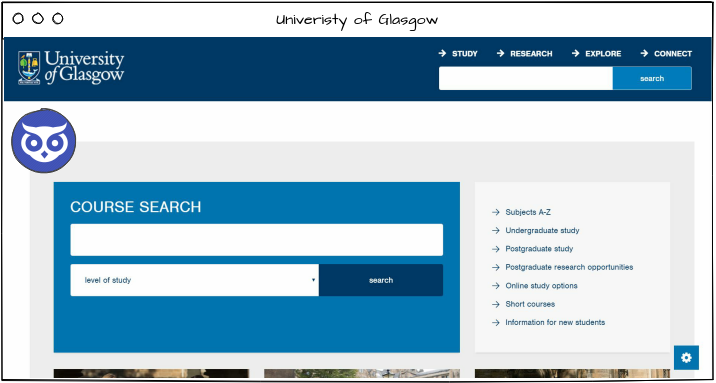
\includegraphics[scale=0.7]{images/Chatbot_w1.png}

\begin{figure}[H]
    \centering
    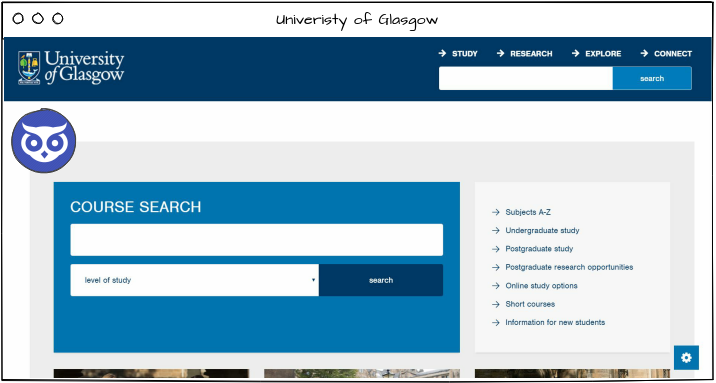
\includegraphics[scale=0.7]{images/Chatbot_w1}
    \caption{Initial Wireframe 1}
    \label{fig:wireframe1}
\end{figure}

\begin{figure}[H]
    \centering
    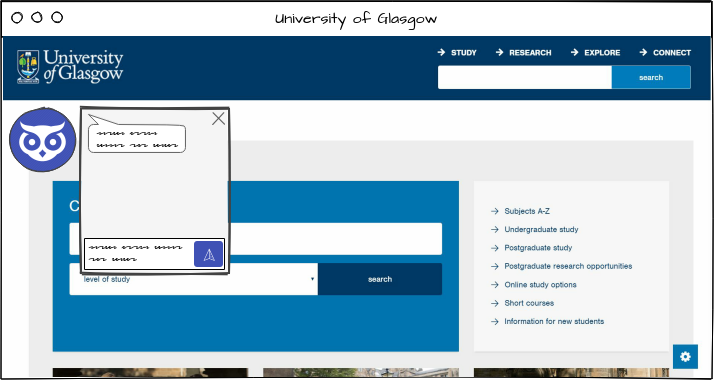
\includegraphics[scale=0.7]{images/Chatbot_w3}
    \caption{Initial Wireframe 2}
    \label{fig:wireframe2}
\end{figure}

\begin{figure}[H]
    \centering
    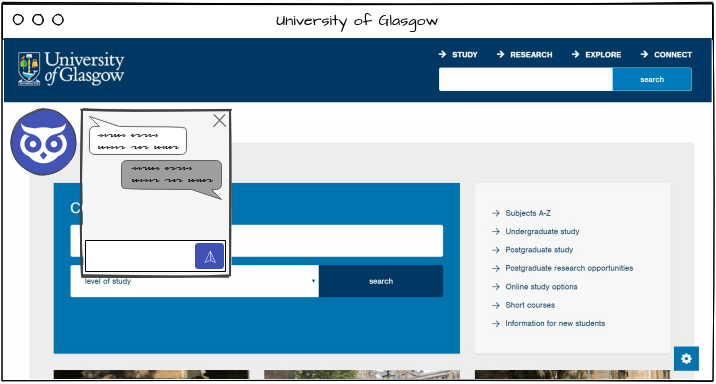
\includegraphics[scale=0.7]{images/Chatbot_w2}
    \caption{Initial Wireframe 3}
    \label{fig:wirefram3}
\end{figure}

\section{Eduroam Blocking Port 3306 Diagnosis}
The command that was used to determine that port 3306 was blocked is shown in figure 4. The command outputs all ports that are open, and since 3306 is not printed out, it is logical to assume that is is blocked.

\begin{figure}[H]
    \centering
    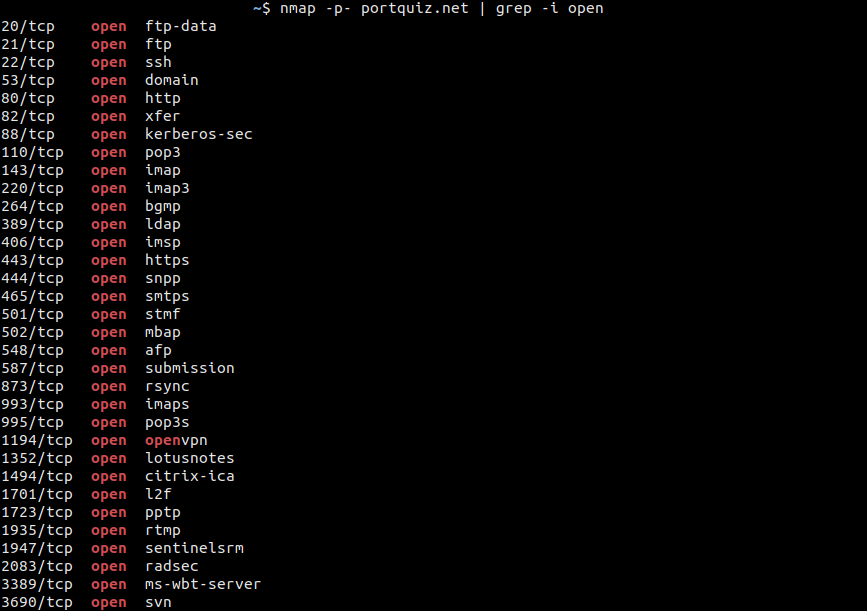
\includegraphics[scale=0.5]{images/eduroam_blocking_3306}
    \caption{Eduroam Blocking Port 3306}
    \label{fig:eduroam}
\end{figure}

\section{Supplemental Testing Information}
\subsection{Dialogflow}
Dialogflow does not have its own testing tool. The team tested it by compiling a list of possible questions posed by the user and the intent Dialogflow was expected to detect and wrote unit tests using Cypress to test these through the front-end.

\subsection{Firebase}
Firebase HTTPS callable functions are not officially testable. Due to this, the team unfortunately could not write unit tests for the function.



\end{document}
